\documentclass[12pt]{article}
\setlength{\oddsidemargin}{0in}
\setlength{\evensidemargin}{0in}
\setlength{\textwidth}{6.5in}
\setlength{\parindent}{0in}
\setlength{\parskip}{\baselineskip}

\usepackage{amsmath,amsfonts,amssymb,graphicx,enumerate,float}

\begin{document}

CSCI 5454 \hfill Problem Set 4\\
Robert Werthman\\
No Collaborators

\hrulefill

\begin{enumerate}
  \item \textit{Implement the action setting of Hedge and use it to complete a
  few tasks.}
  	\begin{enumerate}
  	  \item \textit{Use Hedge to write a game AI and display some sample output.}
  	    \scriptsize
  	  	\begin{verbatim}
	 	Payoff Matrix
		[-8, 10, 2]
		[-4, -2, -1]
		[-8, -6, 1]
		##########
		Round 0
		##########
		Enter the row you wish to choose: 0
		Action chosen by user 0
		Probability distribution of AI actions [0.3333333333333333,0.3333333333333333,0.3333333333333333]
		Action chosen by AI 1
		AI loss vector [-8, 10, 2]
		AI weight vector [2980.9579870417283, 4.5399929762484854e-05, 0.1353352832366127]
		old AI score 0.0 , new AI score -10.0 , difference -10.0
		old user score 0.0 , new user score 10.0 , difference 10.0
		##########
		Round 1
		##########
		Enter the row you wish to choose: 0
		Action chosen by user 0
		Probability distribution of AI actions [0.9999545869027009, 
		1.522928810416062e-08, 4.5397868011057175e-05]
		Action chosen by AI 0
		AI loss vector [-8, 10, 2]
		AI weight vector [8886110.520507872, 2.061153622438558e-09, 0.018315638888734182]
		old AI score -10.0 , new AI score -2.0 , difference 8.0
		old user score 10.0 , new user score 2.0 , difference -8.0
		##########
		Round 2
		##########
		Enter the row you wish to choose: 0
		Action chosen by user 0
		Probability distribution of AI actions [0.9999999979388461,2.319522825462676e-16,2.0611536181902033e-09]
		Action chosen by AI 0
		AI loss vector [-8, 10, 2]
		AI weight vector [26489122129.84347, 9.357622968840175e-14, 0.002478752176666359]
		old AI score -2.0 , new AI score 6.0 , difference 8.0
		old user score 2.0 , new user score -6.0 , difference -8.0
  		\end{verbatim}
  	  	\normalsize
  	  \item \textit{Give a plot that exhibits $\Theta{(\sqrt{T})}$ regret.}
  	    \begin{figure}[H]
  	    \centering
  	    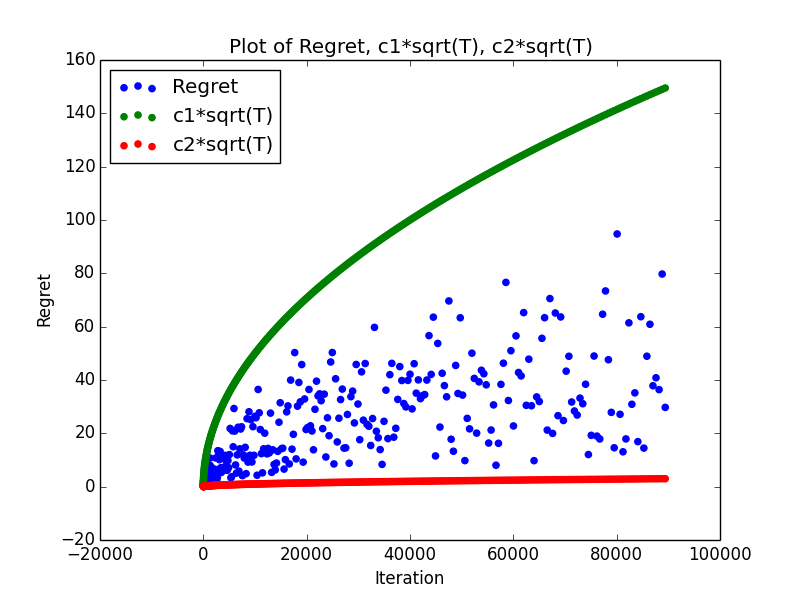
\includegraphics[width=9cm]{q1b.png}
  	    \end{figure}
  	    I let $c_1 = .5$ and $c_2 = .01$ and $\eta = \sqrt{\frac{8ln\,N}{T}}$. 
  	    The graph shows that regret is bounded by $\Theta{(\sqrt{T})}$ where T is the number of rounds. Regret remained
  	    $\le \sqrt(\frac{T}{2}ln\,N)$.  At times regret would get really close to
  	    the bound but other times it would not be close.  It never went above the
  	    bound. Example output of regret in the first column and
  	    $\sqrt(\frac{T}{2}ln\,N)$ in the second column is below.
  	    \scriptsize
  	    \begin{verbatim}
		0.0854754326956 1.16388787282
		0.711207959794 1.55185049709
		0.915738476176 1.93981312136
		1.86659059913 2.32777574563
		1.11868740447 2.7157383699
		0.942107984927 3.10370099418
		1.20108924348 3.49166361845
		2.33209799223 3.87962624272
		2.39799236386 4.26758886699
		3.71141140061 4.65555149126
		3.10138106514 5.04351411554
		1.19507429131 5.43147673981
		3.95892727292 5.81943936408
		0.926603427611 6.20740198835
		2.69832933191 6.59536461262
		0.594289924894 6.9833272369
		6.25916816147 7.37128986117
		3.62512254793 7.75925248544
		0.855690231446 8.14721510971
  	    \end{verbatim}
  	    \normalsize
  	\end{enumerate}
  \item
  \item
  \item
  \item \textit{Find a mixed nash equilibrium of the zero-sum game.  Give both
  strategies and the value of the game and show the vector of expected payoffs
  for player 2 under player 1's strategy and vice versa.}
    $$
    M = \begin{bmatrix}
        1 & 0 & 1 & 8 & 0\\
        5 & 8 & 9 & 2 & 1\\
        0 & 1 & 8 & 0 & 5\\
        8 & 9 & 2 & 1 & 0\\
        1 & 8 & 0 & 5 & 8\\
        \end{bmatrix}
    $$
    
\end{enumerate}


\end{document}